\documentclass[12pt]{report}

\usepackage{fullpage}
\usepackage{amsmath,amssymb,bm,upgreek,mathrsfs}
\usepackage{algorithmic,algorithm}
\usepackage{graphicx,subcaption}
\usepackage{setspace}
\usepackage{color}
\usepackage{multirow}
\usepackage{alltt}
\usepackage{cancel}
\usepackage{listings}

\doublespacing

\DeclareMathOperator*{\argmax}{arg\,max}
\DeclareMathOperator*{\argmin}{arg\,min}

\newcommand{\N}{\mathcal{N}} \newcommand{\U}{\mathcal{U}}
\newcommand{\Poi}{{\text Poisson}} \newcommand{\Exp}{{\text Exp}}
\newcommand{\G}{\mathcal{G}} \newcommand{\Ber}{{\text Bern}}
\newcommand{\Lap}{{\text Laplace}} \newcommand{\btheta}{\boldsymbol{\theta}}
\newcommand{\bSigma}{\boldsymbol{\Sigma}}

\newcommand{\E}[1]{\mathbb{E}[#1]}
\newcommand{\Cov}[2]{\mathbb{C}\mathrm{ov}(#1,#2)}

\def\*#1{\mathbf{#1}} \newcommand*{\V}[1]{\mathbf{#1}}

%%%%%%%%%%%%%%%%%%%%%%%%%%%%%%%%%%%%%%%%%%%%%%%%%%%%%%%%%%%%%%%%%%%%%%

\begin{document}

\centerline{\it CS 477 HW \#13}
\centerline{Questions completed: All undergrad level questions in MATLAB}

\begin{enumerate}

\item[A.] Computing disparity between image locations.

  Below in Figure 1, the two disparity maps for the two pairs of left/right
  images are shown.

  \begin{figure}[H]
    \centering
    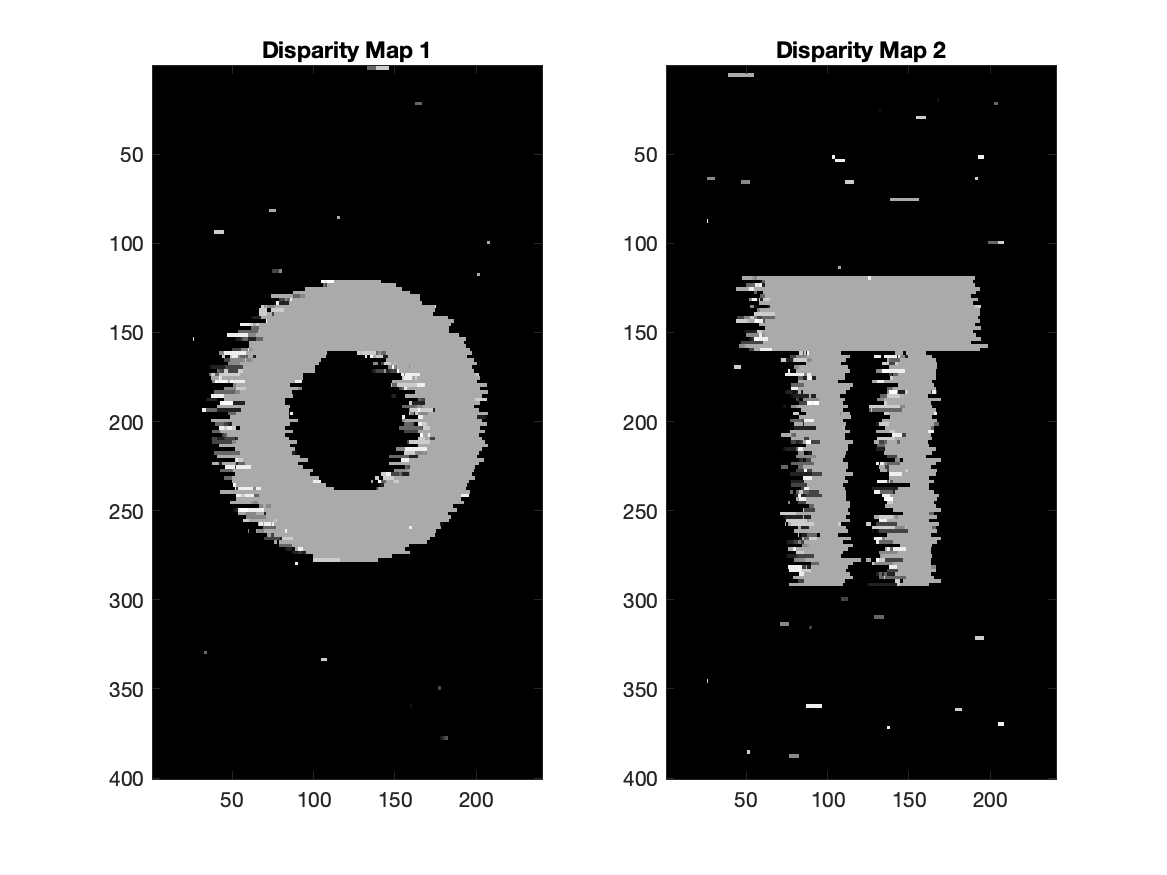
\includegraphics[width=\linewidth]{a1.png}
    \caption{The two disparity maps for the two pairs of left/right random dot
      stereograms given in the assignment are shown using
      \texttt{imagesc()}. The disparity map on the left is for the left1/right1
      pair and the disparity map on the right is for the left2/right2
      pair. Black pixels indicate no disparity while lighter pixels indicate
      more disparity, up to a maximum of 15 pixels in disparity.}
  \end{figure}

  The disparity map was computed as suggested in the assignment. The margins
  were avoided with the suggested row indexing method. In particular,
  \( D = 15\) was set as the maximum disparity distance, and \( C = 10\) was set
  as the number of local pixels on both sides of the current pixel to make
  disparity matches of 21-length row vectors. This gave a total margin of
  \( D + C = 15 + 10 = 25\). Additionaly, the row vectors were normalized before
  taking their dot product if their sum did not equal zero. The absolute value
  of the disparity value that gave the highest dot product was recorded in a
  matrix for each pixel, and the resulting disparity map matrices for both pairs
  of stereograms were displayed using \texttt{imagesc()} which took care of
  scaling the disparity values for display.

  The single interesting distance relative to the background for each pair of
  stereograms is reported as follows.

\begin{verbatim}
Average disparity (set 1): 10.3035
Average disparity (set 2): 10.3275
\end{verbatim}

  The interesting distance was calculated by averaging the top 10\% of the
  largest absolute value disparities in the disparity map for both sets.

  The distance associated with the surface for each set is reported as follows.

\begin{verbatim}
Estimated distance (set 1): 77.6432 cm
Estimated distance (set 2): 77.4631 cm
\end{verbatim}

  This distance was calculated using the equation in the slides
  \( z = f*\frac{d-D}{D}\) for focal length \( f=2cm\), inter-ocular distance
  \( d = 10cm\), pixel size \( p = 0.025cm\), disparity
  \(D = (average\ disparity) * (pixel\ size) = 10.3*0.025cm \approx 0.25cm\),
  and \( (d-D) \approx d\) as the assignment suggested that \(D \ll
  d\). However, I thought that \(D \ll d\) did not hold in my case since
  \( D \approx 0.25cm\) and \( d = 10cm\) for both sets, so I recomputed \(z\)
  with \(d-D\) to get the following.

\begin{verbatim}
Estimated distance (set 1): 75.6432 cm
Estimated distance (set 2): 75.4631 cm
\end{verbatim}

  It appears that the distance is \(2cm\) lower compared to the calculation with
  the \( (d-D) \approx d\) assumption. It seems that either calcuation is fine
  according to a post on Piazza discussing this.

\item[B.] Measuring how far away a star is.

  For focal length \(f=2m\), inter-ocular distance
  \(d=80,000,000\ miles * \frac{1,609.344 m}{mile} = 1.2875*10^{11}m\), and
  disparity \(D=6.2*10^{-6}m\), the distance calcuation in miles is as follows.

  \[z=\frac{f*d}{D}\]
  \[z=\frac{(2m)*(1.2875\times 10^{11}m)}{6.2\times 10^{-6}}\]
  \[z=(4.1531\times 10^{16}m) * \frac{1\ mile}{1,609.344m}\]
  \[z=2.5806\times 10^{13}\ miles\]

  The conversion to from miles to light-years is as follows.

  \[z=(2.5806\times 10^{13}\ miles) * \frac{1\ light\text{-}year}{5.879\times
      10^{12}}\]
  \[z=4.3896\ light\text{-}years\]

  According to the table of nearest stars from the Wikipedia page linked in the
  assignment, the star that we observed would be either Rigil Kentaurus or
  Toliman in the Alpha Centauri star system with a listed distance of 4.3441
  ±0.0022 light-years for both. It was clarified in a Piazza post discussion
  that Rigil Kentaurus and Toliman are a binary pair, and early experiments
  could have treated them as a single star.

  %TODO: list recorded distance and margins of error and talk about how the
  %calcuation might have been off

% \item[A.] Finding a line using RANSAC.

%   Below in Figure 1, the homogeneous least squares best fit line found using
%   RANSAC is shown.

%   \begin{figure}[H]
%     \centering
%     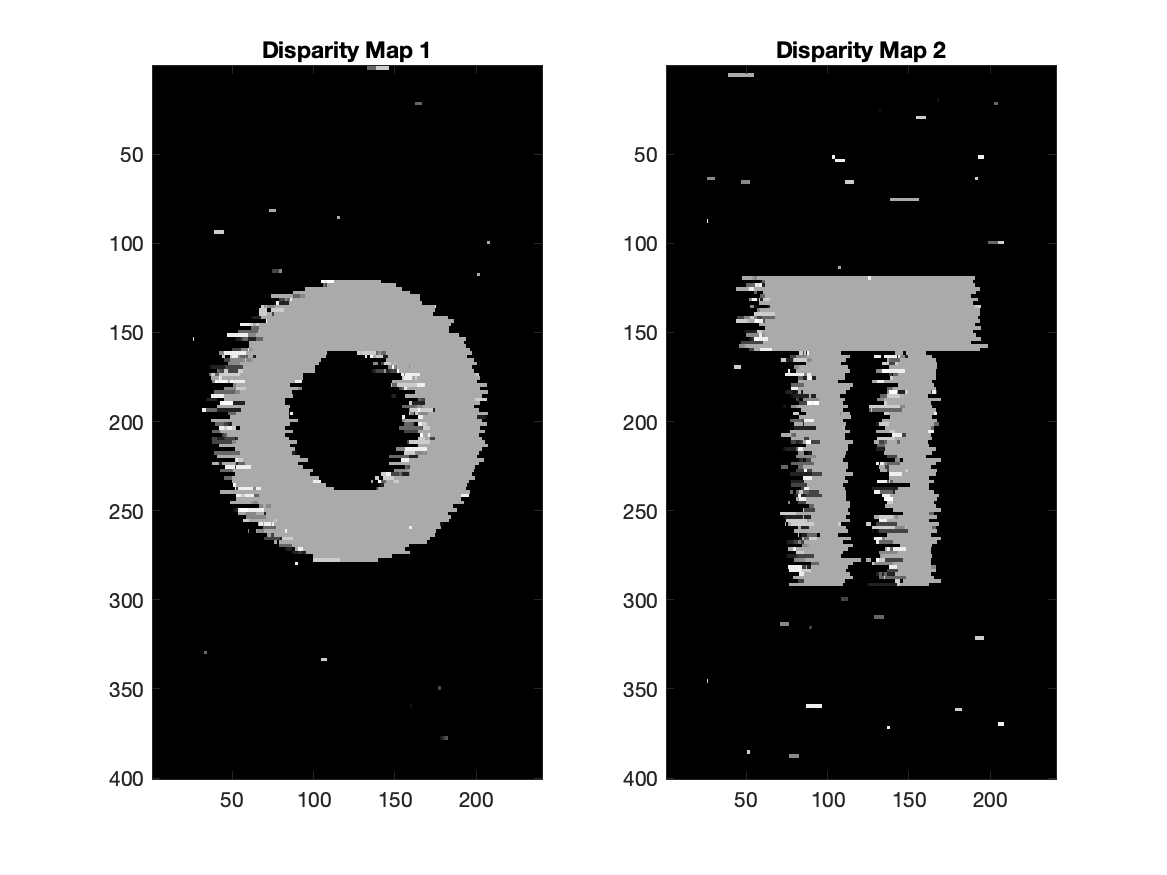
\includegraphics[width=\linewidth]{a1.png}
%     \caption{The homogeneous least squares best fit line was found using the
%       RANSAC algorithm. The number of iterations for the RANSAC algorithm to
%       find this line was \( K = \log(1-0.9999)/\log(1-0.25^2) \approx 143\)
%       where \( 0.9999\) is the probability of a valid fit, \( 0.25\) is the
%       probability of getting an inlier (because the problem specified that a
%       quarter of the points lie on a line), and the squared is from the minimum
%       number of points needed for the model (two points to form a line).}
%   \end{figure}

%   In the RANSAC algorithm for each iteration, two random points to form a line
%   were selected, and the inliers were assigned to the top 25\% of points
%   perpendicular to the random line. After the inliers were found, the line was
%   refitted using homogeneous least squares on the inliers, and then the error was
%   computed by taking the sum of the squared perpendicular distances of the
%   inliers to the refitted line. The best error turned out to be \( 0.2576\)
%   which came from the best fit line with a slope of \( -0.4895\) and an
%   intercept of \( 2.0023\).

%   A plot was then generated as shown above in Figure 1 using MATLAB functions
%   \texttt{scatter()} and \texttt{plot()}. From visual inspection, it appears
%   that the RANSAC algorithm was effective in identifying the quarter of points
%   that were spread along a good line.

% \item[B.] Implementing DLT method for computing homography between two planar
%   images.

%   The RMS error of the transformation for 4, 5, and 6 randomly generated pairs
%   of points inside [0,1]x[0,1] over 10 samples using homography is reported
%   below (from left to right).

% \begin{verbatim}
%   RMSE_samples =
%   0.0000    0.1811    1.1338
% \end{verbatim}

%   My results suggest that the code is working because I would expect the RMSE to
%   increase with the number of points that is used in homography computation when
%   we are working purely with randomly generated ``pairs'' of points.

%   I also reran the code several times for good measure since we are working with
%   randomly generated pairs, and the results are what is expected most of the
%   time, with the occasional case of 6 random pairs getting a lower RMSE than 5
%   random pairs (but this is also within expectations of working with random
%   pairs). I also tested that my DLT method for computing homography was mapping
%   things correctly before working with randomly generated pairs.
% \newpage
%   Below in Figure 2, the DLT homography testing for each slide/frame pair is
%   shown.

%   \begin{figure}[H]
%     \centering
%     \begin{subfigure}{0.44\linewidth}
%       \includegraphics[width=\linewidth]{b1.png}
%       \caption{slide1 w/ red/cyan clicked stars.}
%     \end{subfigure}
%     \begin{subfigure}{0.44\linewidth}
%       \includegraphics[width=\linewidth]{b2.png}
%       \caption{frame1 w/ red/cyan clicked stars and green mapped dots.}
%     \end{subfigure}
%     \begin{subfigure}{0.44\linewidth}
%       \includegraphics[width=\linewidth]{b3.png}
%       \caption{slide2 w/ red/cyan clicked stars.}
%     \end{subfigure}
%     \begin{subfigure}{0.44\linewidth}
%       \includegraphics[width=\linewidth]{b4.png}
%       \caption{frame2 w/ red/cyan clicked stars and green mapped dots.}
%     \end{subfigure}
%     \begin{subfigure}{0.44\linewidth}
%       \includegraphics[width=\linewidth]{b5.png}
%       \caption{slide3 w/ red/cyan clicked stars.}
%     \end{subfigure}
%     \begin{subfigure}{0.44\linewidth}
%       \includegraphics[width=\linewidth]{b6.png}
%       \caption{frame3 w/ red/cyan clicked stars and green mapped dots.}
%     \end{subfigure}
%     \caption{Clicked point pairs used in DLT homography are shown as red stars
%       in the slide/frame pairs (4 red stars per slide/frame), clicked point
%       pairs not used in homography are shown as cyan stars in the slide/frame
%       pairs (4 cyan stars per slide/frame), and the mapped points from DLT
%       computed homography are shown as green dots on the frames (8 green dots
%       per frame).}
%   \end{figure}

%   From Figure 2 above, one can see that all mapped points (green dots) from DLT
%   homography are relatively close to the clicked points (red/cyan stars) in each
%   frame. Specifically, the green dots in each frame are directly on top of their
%   corresponding red stars since these were the clicked point pairs used for
%   homography. The green dots are also relatively close to their corresponding
%   cyan star clicked points which were not used in homography.

%   Initially, I had terrible homography for the cyan star point pairs (the green
%   dots were nowhere near their corresponding cyan star points) because I naively
%   used the first four out of the eight clicked point pairs for each slide/image
%   which did not give a good spread of points to work with for homography. My
%   solution to this was to use every other point pair in the list of eight as my
%   four point pairs for homography, and it worked out well and resulted in Figure
%   2. Next time, I would make sure to select four point pairs in the slide/frame
%   pairs that fit more to the dimensions of the slides.
% \newpage
% \item[C.] Using RANSAC to improve keypoint matching.

%   Homography with RANSAC improves keypoint matching based on my findings and by
%   a visually significant margin compared to my results from assignment 9. Below
%   in Figure 3, the results of homography with RANSAC to improve keypoint
%   matching of SIFT vectors is shown.

%   \begin{figure}[H]
%     \centering
%     \begin{subfigure}{0.52\linewidth}
%       \includegraphics[width=\linewidth]{c1.png}
%       \caption{slide/frame 1 w/ green dot keypoint matches (homography inliers)
%         connected by red lines.}
%     \end{subfigure}
%     \begin{subfigure}{0.52\linewidth}
%       \includegraphics[width=\linewidth]{c2.png}
%       \caption{slide/frame 2 w/ green dot keypoint matches (homography inliers)
%         connected by red lines.}
%     \end{subfigure}
%     \begin{subfigure}{0.52\linewidth}
%       \includegraphics[width=\linewidth]{c3.png}
%       \caption{slide/frame 3 w/ green dot keypoint matches (homography inliers)
%         connected by red lines.}
%     \end{subfigure}
%     \caption{The results of homography with RANSAC to improve keypoint matching
%       of SIFT vectors from the slide/frame pairs of assignment 9 are shown. The
%       green dots in the slide/frame pairs represent the keypoint matches that
%       were in the homography inliers, and the red lines connecting the green
%       dots signify the matching pairs.}
%   \end{figure}

%   As seen in Figure 3 above, the homography inliers used as the final keypoint
%   matches betweeen slide/frame pairs seem to work well in that there are plenty
%   of keypoint matches produced in each slide/frame pair and in that there are
%   (from visual inspection) no incorrect keypoint matches whatsoever. This is
%   noticeably better than any method used in assignment 9 to narrow down the
%   matches because, from my experiments for that assignment, the vast majority of
%   matches had to be discarded just to get a couple accurate matches for each
%   slide/frame. In contrast, with RANSAC and homography, we see so many more
%   accurate matches now that were missing before.

%   The parameters for the number of iterations was 99.9999\% probability of
%   finding the correct fit, 8\% probability of finding a correct keypoint match
%   (percentage that are homography inliers), and a minimum of 4 keypoint matches
%   required for a fit. Using the number of iterations equation, this resulted in
%   337,286 iterations per slide/frame pair to produce the homography inlier
%   keypoint matches as seen above in Figure 3.

%   Before using homography with RANSAC, \texttt{knnsearch()} was used to produce
%   keypoint matches from the SIFT files from assignment 9 by getting the nearest
%   neighbor for all SIFT points in the slide for all SIFT points in the frame. In
%   each iteration of RANSAC, 4 keypoint matches were randomly chosen in an
%   indefinite while-loop which would not break until all 4 keypoint matches were
%   unique. Then, homography was computed from the four points and then refit to
%   the top 8\% of inliers found based on squared error of the homography versus
%   the frame keypoints. The RMSE of the refitted homography was computed, and the
%   homography inliers were saved if the RMSE was the best one seen so far.

%   Overall, homography with RANSAC produced better results than my methods in
%   assignment 9, and I think the fact that the tuning parameters used to
%   determine the number of iterations is so straight-forward makes this method
%   easier to use. The downside is that the number of iterations for RANSAC could
%   become quite large depending on the parameters, but it seems that at least for
%   the slide/frame pairs that we are using, the results will be more reliable.

\end{enumerate}

\end{document}
